\documentclass{article}
\usepackage[utf8]{inputenc}  % UTF-8 인코딩 지원
\usepackage[a4paper, margin=1in]{geometry}  % 페이지 여백 설정
\usepackage{titlesec}  % 제목 스타일 조정 패키지
\usepackage{titling}   % 제목 추가 스타일링 지원
\usepackage{graphicx}  % 그래픽 삽입을 위한 패키지
\usepackage{caption}   % 캡션을 위한 패키지
\usepackage{subcaption} % 서브캡션 사용을 위한 패키지
\usepackage{array}     % 표 스타일 조정을 위한 패키지
\usepackage{booktabs}  % 더 좋은 표 스타일을 위한 패키지

% 제목 스타일 조정
\pretitle{\begin{center}\LARGE\bfseries}  % 제목 크기와 굵기 (줄임)
\posttitle{\par\vskip 1em\hrule\vskip 1em\end{center}}  % 제목 아래 라인 추가
\preauthor{\begin{center}\normalsize}  % 작성자 정보 크기 조정
\postauthor{\par\end{center}}
\predate{\begin{center}\itshape}  % 날짜 스타일 조정
\postdate{\par\end{center}}

\title{\textbf{\MakeUppercase{Impact of Data Transformations on Model Accuracy:}\\ \MakeUppercase{Homography and Gaussian Noise}}}  % 제목을 대문자로 변경
\author{
    Minwon Lee \\  % 이름
    Department of Automotive Engineering \\  % 학과명
    Hanyang University \\  % 대학명
    Seoul, South Korea  % 위치
}
\date{\textit{\MakeUppercase{December 6, 2024}}}  % 날짜 대문자

\begin{document}

\maketitle  % 제목, 작성자, 날짜 출력

\begin{abstract}  
    This report evaluates the robustness of various machine learning models, 
    including Logistic Regression, SVM, MLP, and CNN, under two types of data transformations: Homography and Gaussian Noise. 
    These transformations are applied to test the models' performance under challenging conditions. 
    Experimental results show that CNN consistently outperformed other models in handling both homography transformations and Gaussian noise, while simpler models like Logistic Regression struggled with increased transformation severity. 
    The findings highlight key considerations for improving model robustness in various data distortion scenarios. 
\end{abstract}

\section{Problem Setting}
This study evaluates the robustness of several machine learning models, including Logistic Regression, Fisher Discriminant Analysis (FDA), Support Vector Machines (SVM), Multilayer Perceptron (MLP), and Convolutional Neural Networks (CNN), under data transformations such as Homography and Gaussian Noise. 

The models are tested on the MNIST dataset, starting with performance evaluation on the original dataset to establish a baseline. The study then examines how each model's accuracy changes under varying levels of data distortion introduced by the transformations. This analysis highlights the strengths and weaknesses of each model in handling these challenges.

\section{Dataset and Data Split}

\subsection{Dataset Overview}
The dataset used for this study contains 1,797 samples, each represented by 64 features. This dataset consists of numerical data derived from handwritten digits. The dataset is uniformly distributed across 10 unique classes, representing digits from 0 to 9. This uniform distribution ensures that each class has roughly the same number of samples, which contributes to a balanced training process.

\begin{figure}[h]
    \centering
    \begin{subfigure}[b]{0.45\textwidth}
        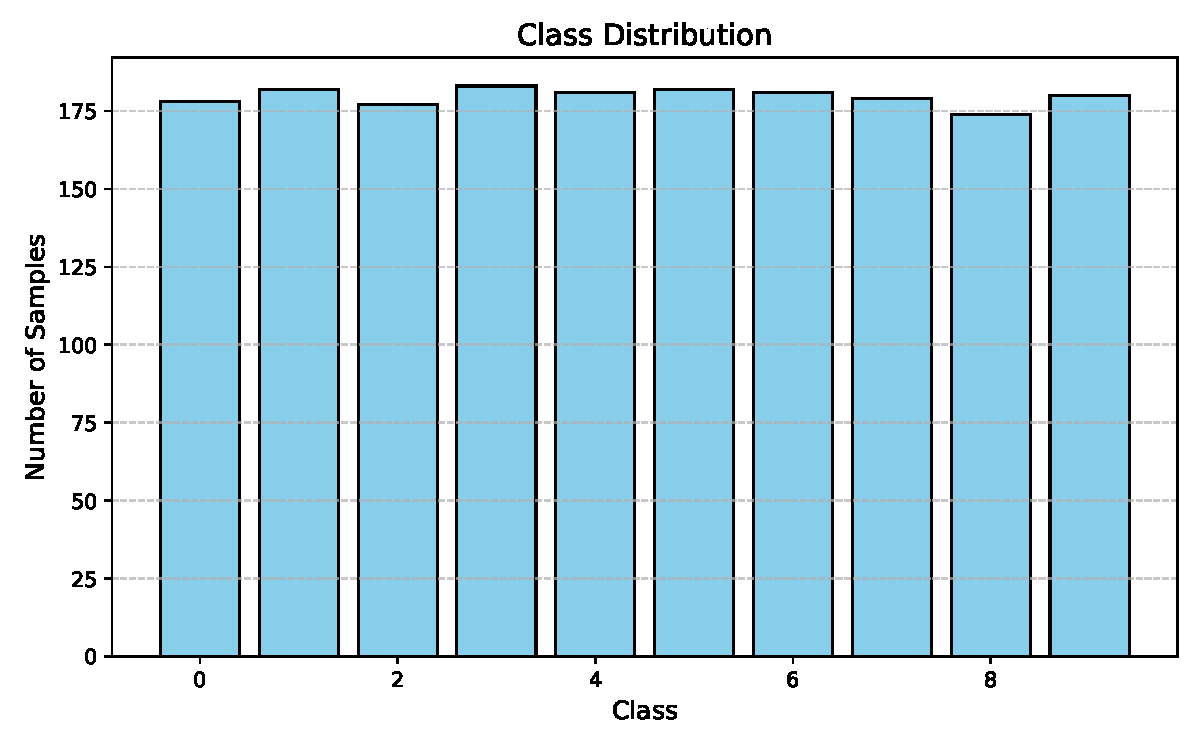
\includegraphics[width=\textwidth]{images/class_distribution.pdf}
        \caption{Class Distribution Visualization}
        \label{fig:class_distribution}
    \end{subfigure}
    \hfill
    \begin{subfigure}[b]{0.45\textwidth}
        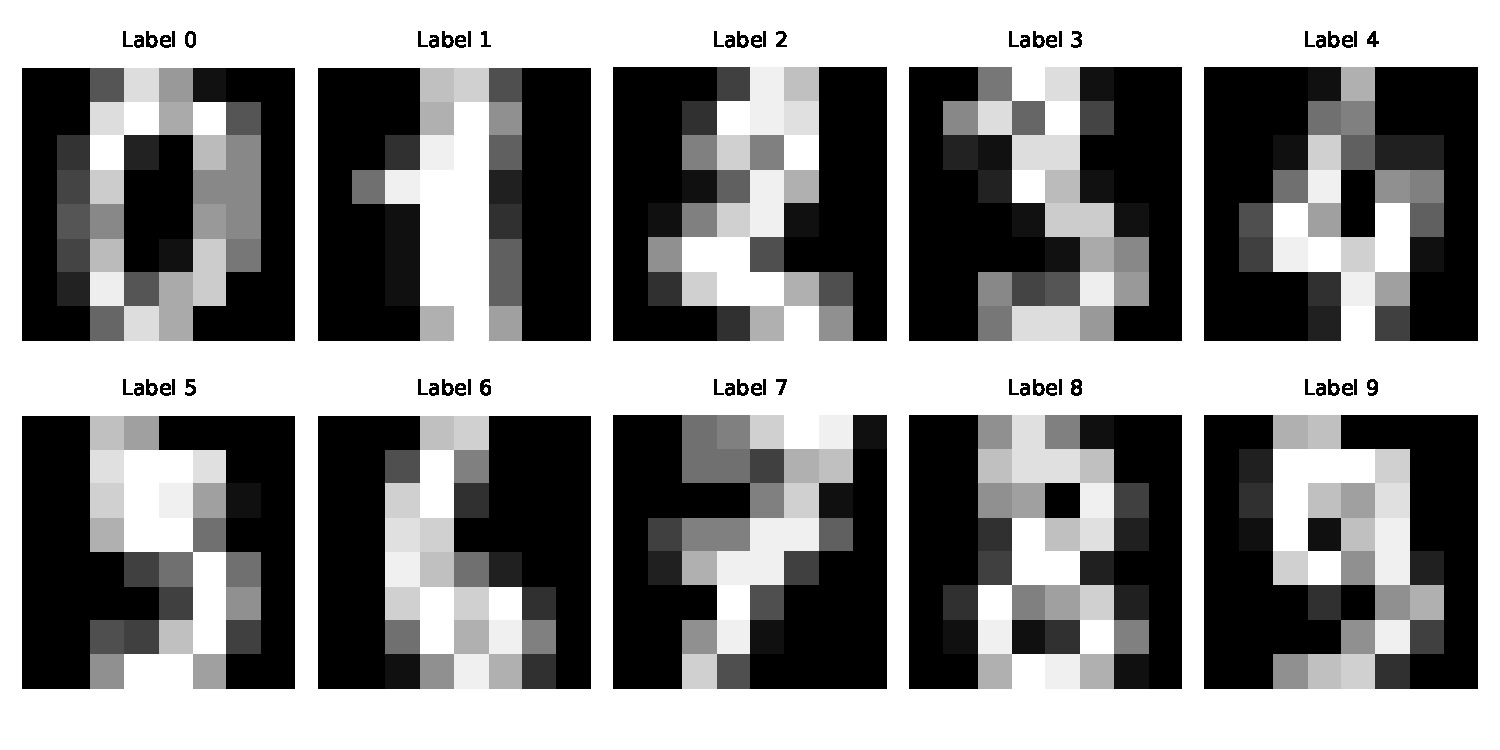
\includegraphics[width=\textwidth]{images/MNIST_samples.pdf}
        \caption{Sample MNIST Images}
        \label{fig:mnist_samples}
    \end{subfigure}
    \caption{Dataset Visualizations: Class distribution and example MNIST images.}
    \label{fig:dataset_visualizations}
\end{figure}

\subsection{Train and Test Data Split}
The dataset is split into training and test sets. The training set contains 1,437 samples, while the test set consists of 360 samples. The test set is reserved for evaluating the generalization performance of the trained model.

\subsection{Train and Validation Split with K-Fold Cross-Validation}
To evaluate model robustness and avoid overfitting, 5-fold cross-validation was applied to the training set. In this method, the training data (1,437 samples) is divided into 5 subsets, where each subset serves as the validation set once while the remaining subsets are used for training. For example, in one fold, 1,149 samples are used for training and 288 samples for validation. This process is repeated across all folds to ensure each data point is used for both training and validation.


\section{Models and Validation Accuracy}

\subsection{Model Overview}
The following machine learning models were used in this study to evaluate their robustness against data transformations. Each model was trained with appropriate hyperparameters and settings to ensure fair evaluation.

\subsubsection{Logistic Regression}
Logistic Regression is a linear model used for binary and multi-class classification. 
The model was trained using the `lbfgs` solver with a maximum of 1,000 iterations. Validation accuracy was computed to evaluate performance.

\subsubsection{Fisher Discriminant Analysis (FDA)}
Fisher Discriminant Analysis (FDA) is a linear discriminant analysis model that projects data to maximize class separability. 
This model was used to examine its capability in handling linearly separable data.

\subsubsection{Support Vector Machine (SVM)}
Two variants of SVM were evaluated in this study. The first used a radial basis function (RBF) kernel, a non-linear classifier effective for capturing complex decision boundaries. The second employed a polynomial kernel of degree 3, enabling it to model interactions between features. 

\subsubsection{Multilayer Perceptron (MLP)}
The MLP model is a simple neural network with one hidden layer containing 100 units, using the ReLU activation function. 

\subsubsection{Multilayer Perceptron (MLP)}
The MLP model is a feedforward neural network designed with three hidden layers containing 128, 64, and 32 units, respectively, each using the ReLU activation function. The model was trained using the Adam optimizer with a learning rate of 0.001 and L2 regularization (alpha = $10^{-4}$) to prevent overfitting. The maximum number of iterations for optimization was set to 1500. Validation accuracy was estimated using 5-fold cross-validation, with training and validation splits determined dynamically.

\subsubsection{Convolutional Neural Network (CNN)}
The CNN is a deep learning model tailored for image data and features the following architecture:
\begin{itemize}
    \item Two convolutional layers with 64 filters each, using a $3 \times 3$ kernel, ReLU activation, and Batch Normalization for stabilization.
    \item A max-pooling layer with a $2 \times 2$ window, followed by a dropout layer with a rate of 0.3.
    \item Two additional convolutional layers with 128 filters each, using a $3 \times 3$ kernel and ReLU activation, followed by another max-pooling layer and a dropout layer with a rate of 0.4.
    \item A fully connected layer with 256 units, followed by a dropout layer with a rate of 0.5, and an output layer with 10 units corresponding to the number of classes.
\end{itemize}
The model was compiled using the Adam optimizer. It was trained for 20 epochs with a batch size of 32. Validation was conducted on 20\% of the training data.

\subsection{Validation Accuracy for Each Model}
The table below summarizes the validation accuracy of each model after training. For Logistic Regression, FDA, SVM, and MLP, validation accuracy represents the average performance across 5-fold cross-validation. For CNN, validation accuracy was computed on a separate validation set (20\% of the training data).

\begin{table}[h]
    \centering
    \caption{Average Validation Accuracy for Each Model}
    \label{tab:validation_accuracy}
    \begin{tabular}{l c}
        \toprule
        \textbf{Model} & \textbf{Average Validation Accuracy} \\
        \midrule
        Logistic Regression & 0.9617 \\
        Fisher Discriminant Analysis (FDA) & 0.9478 \\
        SVM (RBF Kernel) & 0.9861 \\
        SVM (Polynomial Kernel) & 0.9882 \\
        Multilayer Perceptron (MLP) & 0.9763 \\
        Convolutional Neural Network (CNN) & 0.9792 \\
        \bottomrule
    \end{tabular}
\end{table}

The 5-fold cross-validation ensures that each data point in the training set is used for both training and validation, which helps provide a more reliable estimate of the model's performance and minimizes bias.

\section{Experimental Setup}

\subsection{Homography Transformation}
Homography transformations were applied to simulate perspective distortions by randomly shifting the coordinates of the image corners. The maximum offset (\textit{max\_offset}) used to define the range of these random shifts was tested at three levels: 1.5, 2.0, and 2.5 pixels. These progressively severe transformations were designed to evaluate the models' ability to handle perspective changes.

\subsection{Gaussian Noise}
Gaussian noise was added to the images to simulate noisy conditions, commonly encountered in practical scenarios like low-light environments. Noise levels were defined by the standard deviation (\textit{sigma}) of the Gaussian distribution, with three levels tested: 0.2, 0.5, and 0.7. These levels introduced increasing degrees of image degradation to test the robustness of the models.

\subsection{Transformation Visualization}
To provide a qualitative insight into the applied transformations, Figure~\ref{fig:experiment_visualization} illustrates the impact of Homography (max\_offset = 2.5) and Gaussian Noise (sigma = 0.7) on sample images from the dataset. These examples represent the most challenging transformations applied in this study.

\begin{figure}[h!]
    \centering
    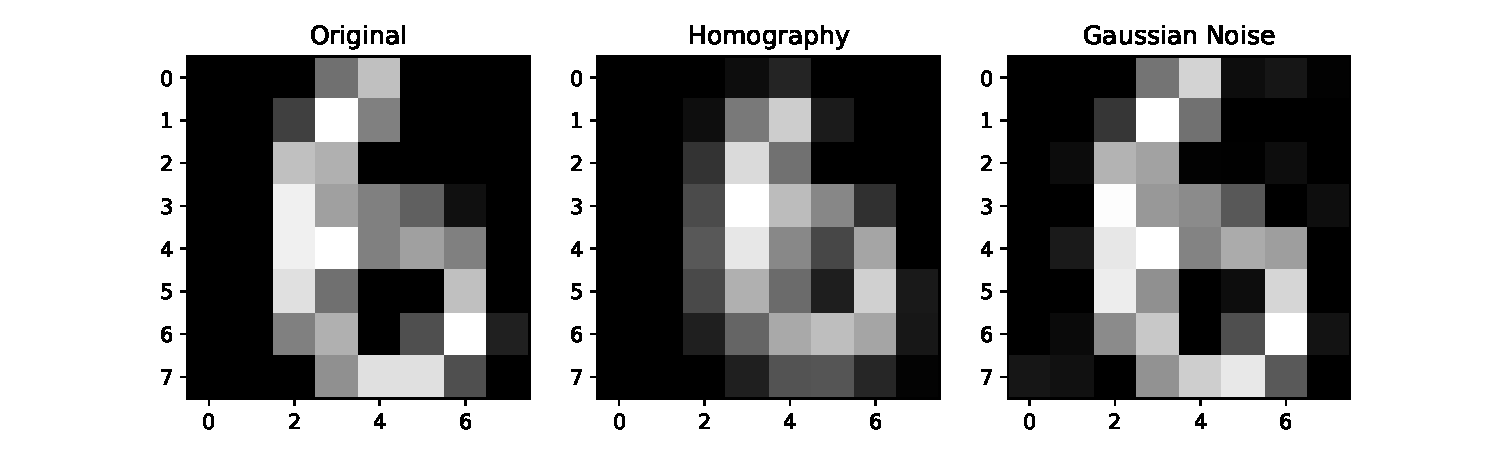
\includegraphics[width=0.8\textwidth]{images/Experiment.pdf}
    \caption{Visualization of Homography Transformation (max\_offset = 2.5) and Gaussian Noise (sigma = 0.7).}
    \label{fig:experiment_visualization}
\end{figure}

\section{Experiment Results}

\subsection{Baseline Accuracy}
The baseline accuracy represents the performance of each model on the original MNIST dataset without any transformations. Table~\ref{tab:baseline_accuracy} summarizes the accuracy for all models, highlighting the effectiveness of CNN and SVM with a polynomial kernel, which achieved the highest accuracy.

\begin{table}[h!]
    \centering
    \caption{Baseline Accuracy for Each Model}
    \label{tab:baseline_accuracy}
    \begin{tabular}{|l|c|}
        \hline
        \textbf{Model} & \textbf{Baseline Accuracy} \\
        \hline
        Logistic Regression & 0.9667 \\
        Fisher Discriminant Analysis (FDA) & 0.9444 \\
        SVM (RBF Kernel) & 0.9861 \\
        SVM (Polynomial Kernel) & 0.9917 \\
        Multilayer Perceptron (MLP) & 0.9778 \\
        Convolutional Neural Network (CNN) & 0.9944 \\
        \hline
    \end{tabular}
\end{table}

\begin{figure}[h!]
    \centering
    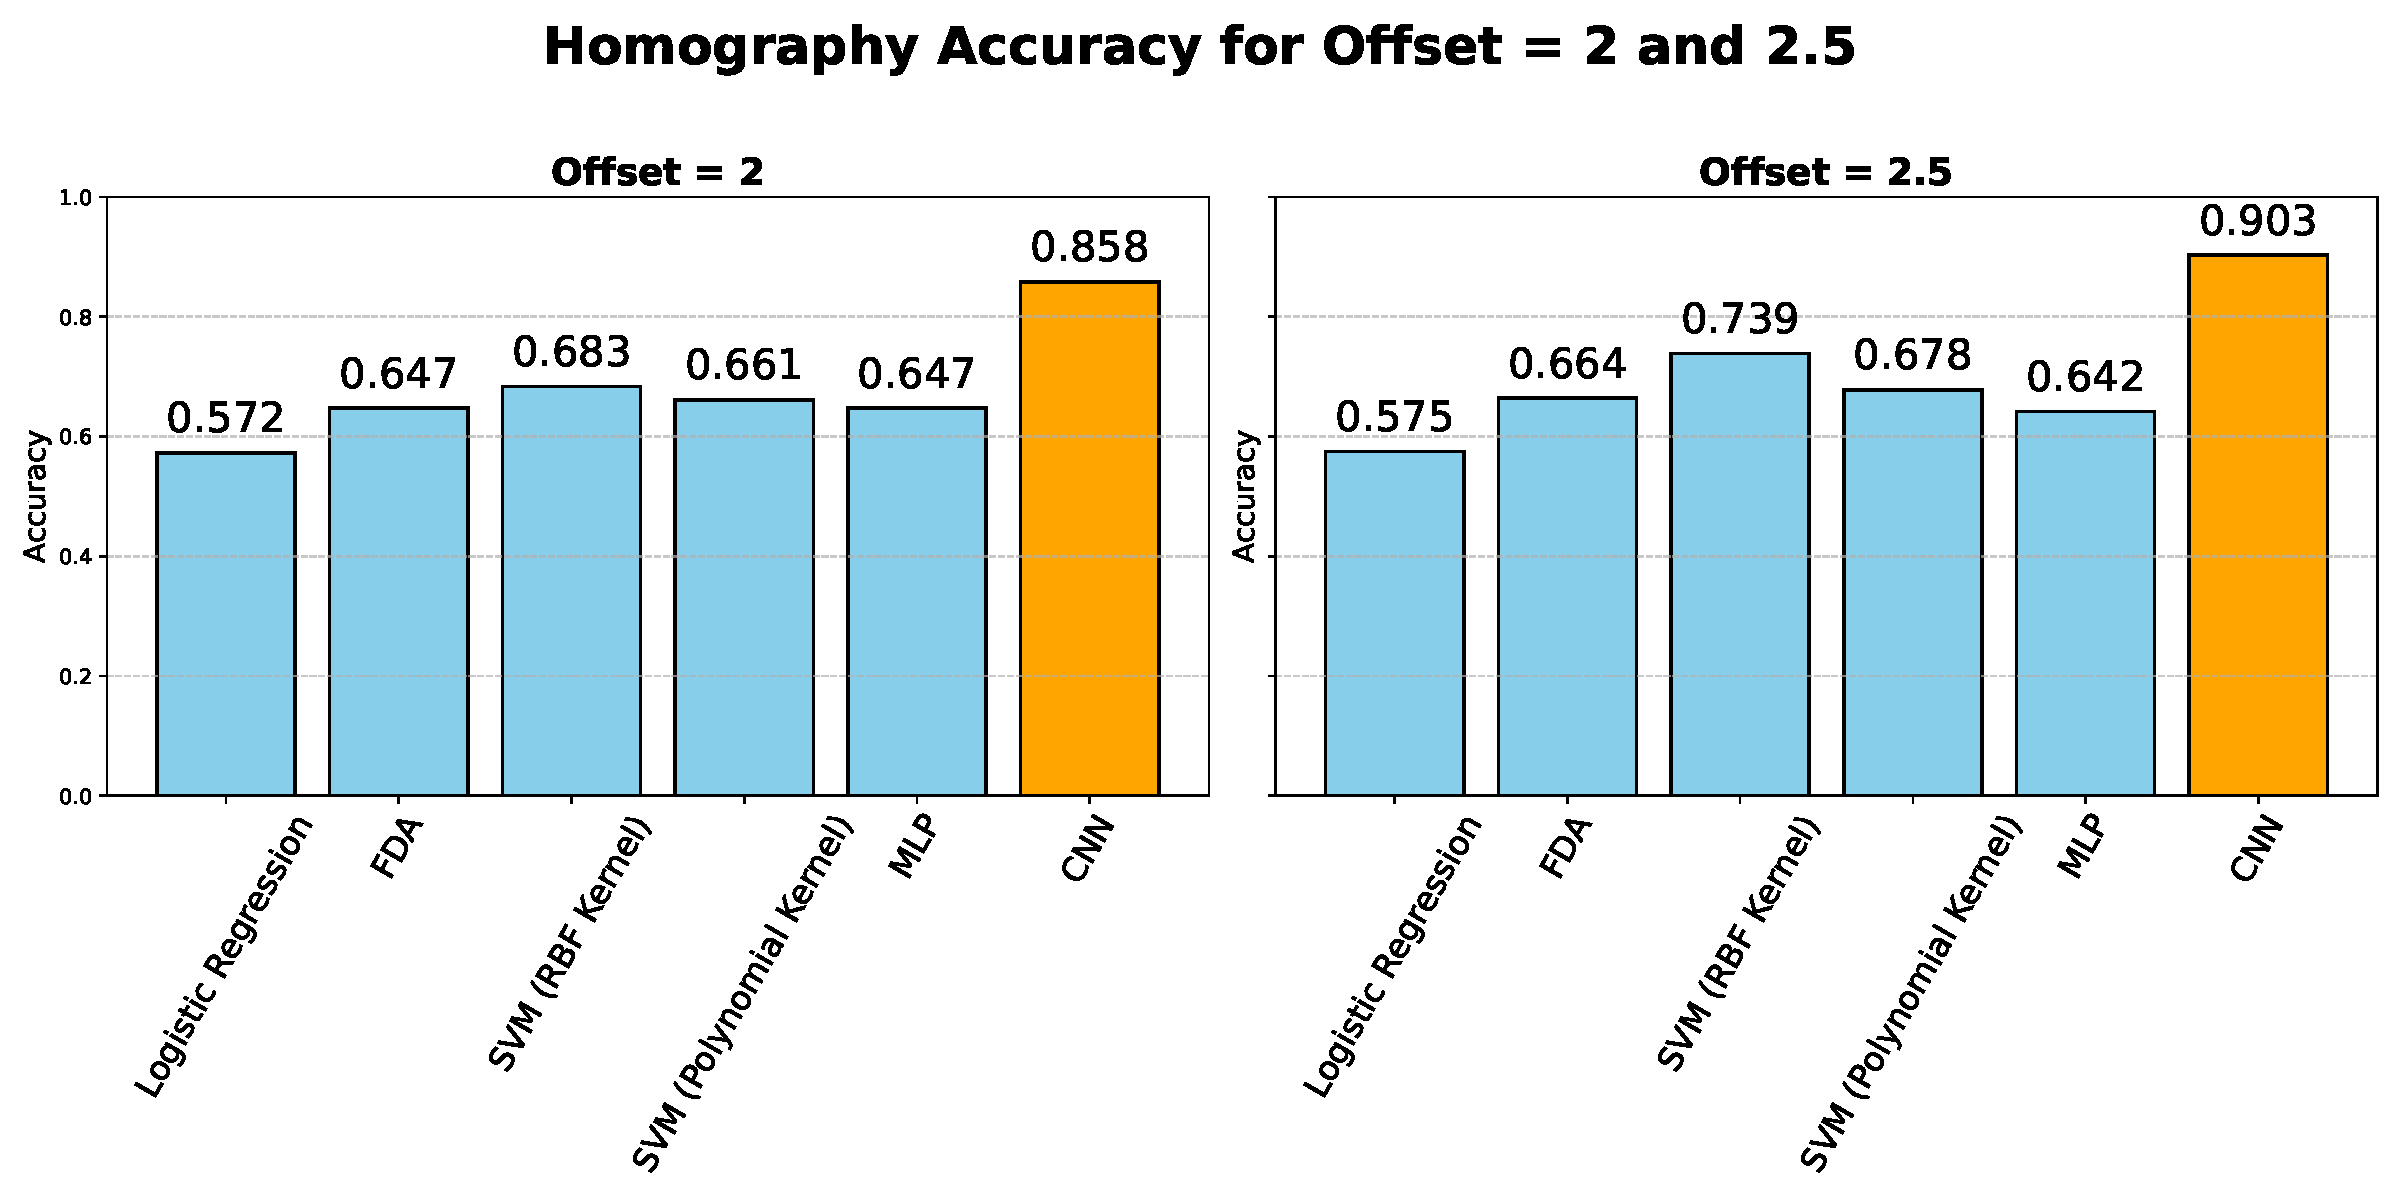
\includegraphics[width=0.8\textwidth]{images/homography.pdf}
    \caption{Accuracy under homography transformations with different max\_offset values.}
    \label{fig:homography_accuracy}
\end{figure}

\begin{figure}[h!]
    \centering
    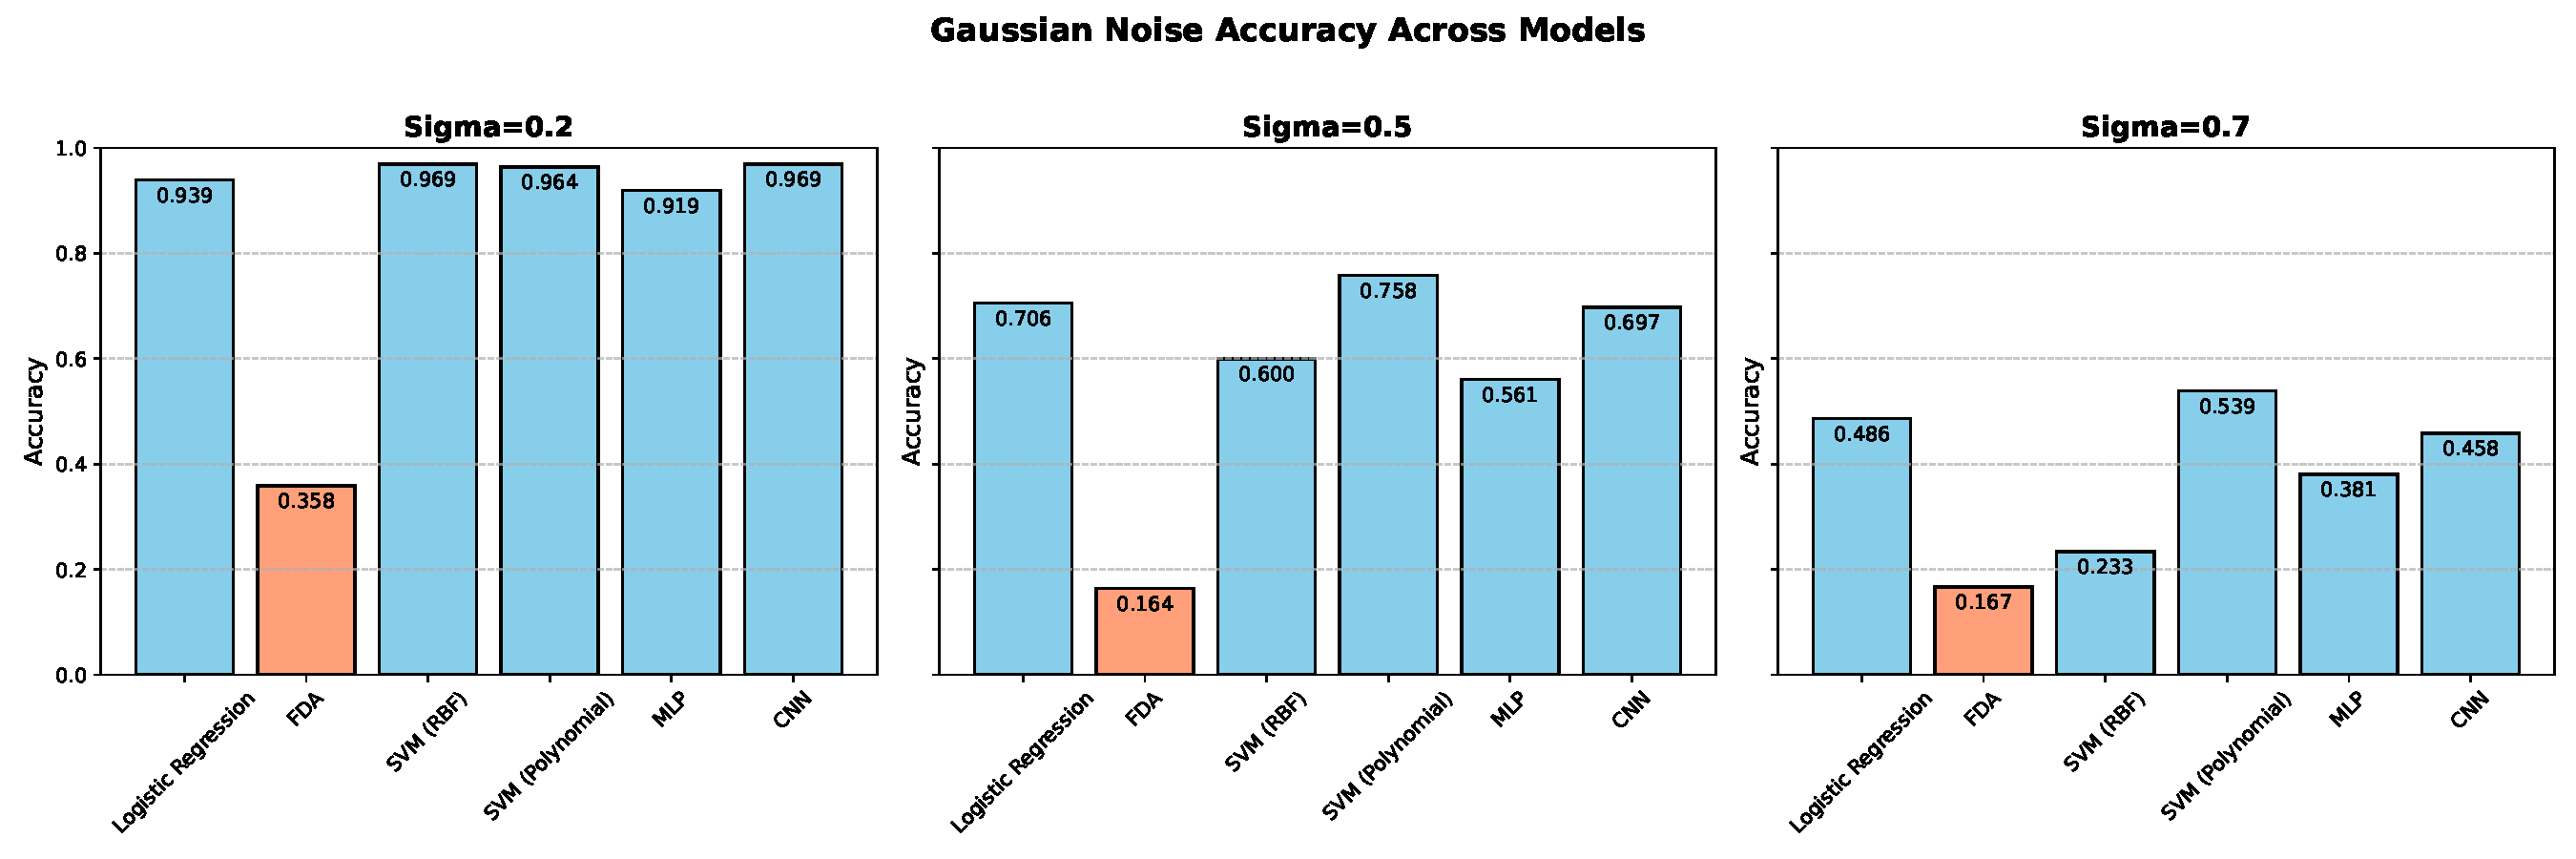
\includegraphics[width=0.8\textwidth]{images/gaussian_noise.pdf}
    \caption{Accuracy under Gaussian noise transformations with different sigma values.}
    \label{fig:gaussian_noise_accuracy}
\end{figure}

\subsection{Analysis and Comparison of Results}

\subsubsection{Performance Analysis for Each Algorithm}
The evaluation results demonstrate clear distinctions in how different algorithms respond to baseline, homography, and Gaussian noise transformations. Key observations include:

\begin{itemize}
    \item \textbf{Baseline Accuracy}: CNN and SVM with a Polynomial Kernel achieved the highest accuracy on the original dataset, indicating their capability to model complex patterns effectively. Logistic Regression also performed well, but FDA lagged behind due to its linear nature.
    \item \textbf{Homography Transformation}: As homography severity increased (max\_offset = 2 and 2.5), CNN consistently outperformed other models, with accuracy levels remaining above 85\% even at the highest offset. SVM with an RBF Kernel also showed notable resilience, whereas Logistic Regression and MLP experienced significant drops in performance.
    \item \textbf{Gaussian Noise}: With increasing noise levels (sigma = 0.5 and 0.7), CNN and SVM with a Polynomial Kernel displayed better tolerance to noise compared to other models. FDA's performance declined dramatically, highlighting its sensitivity to noisy data. Logistic Regression, while performing better than FDA, showed limitations in handling higher noise levels.
\end{itemize}

\subsubsection{Pros and Cons of Each Algorithm}
The models studied can be categorized into three groups based on their design and strengths: linear models, non-linear models, and neural networks. Each category offers unique trade-offs:

\textbf{Linear Models}: Logistic Regression and FDA are efficient for linearly separable data and work well on clean datasets. Logistic Regression demonstrated decent accuracy under baseline conditions but struggled with severe transformations. FDA's performance was significantly impacted by Gaussian noise, making it unsuitable for tasks involving high variability.

\textbf{Non-Linear Models}: SVM with RBF and Polynomial kernels excel at capturing complex data patterns, with SVM (RBF Kernel) showing robust performance under homography transformations. However, these models require careful parameter tuning and become computationally demanding for larger datasets. The Polynomial Kernel displayed strong tolerance to noise but experienced minor accuracy drops with increasing homography severity.

\textbf{Neural Networks}: MLP and CNN excelled in non-linear tasks, with CNN emerging as the most robust model across all scenarios. CNN handled perspective transformations and Gaussian noise better than other models, maintaining relatively high accuracy even under challenging conditions. However, these models are computationally intensive, require large amounts of training data, and are sensitive to hyperparameter choices.

In summary, CNN demonstrated consistent superiority in scenarios involving complex transformations and noise, making it the most robust choice among the evaluated models. However, its computational demands and training requirements make it less practical for applications where efficiency is a primary concern.

\section{Conclusion}

This study evaluated the robustness of six machine learning models (Logistic Regression, FDA, SVM with RBF and Polynomial kernels, MLP, and CNN) under homography and Gaussian noise transformations. These transformations introduced perspective changes and noise, simulating real-world data distortions.

\subsection*{Key Findings}
CNN and SVM with Polynomial Kernel consistently outperformed other models, particularly under baseline and noisy conditions. While CNN demonstrated superior resilience to perspective changes, simpler models like Logistic Regression and FDA were less effective under challenging transformations.

\subsection*{Limitations and Future Work}
This study was limited to the MNIST dataset and two transformation types. Future research should explore more diverse datasets and additional transformations, such as scaling and rotation, to provide a broader evaluation of model robustness.

In summary, this study emphasizes the need to select models based on their robustness to data distortions, ensuring reliable performance in real-world scenarios.

\end{document}

